\chapter{黑洞、白洞與整體因果圖}

\lectureoverview{視界在局部看來平凡，對整體卻至關重要。我們先從近視界的史瓦西度規出發，藉由歐幾里得雪茄的類比向外推展，再來探問愛麗絲和鮑勃實際上能看到什麼。奇點與時間反演的白洞區域，將這幅局部圖像擴展為永恆的史瓦西時空。彭羅斯緊緻化讓因果結構變得有限而易於閱讀。最後，我們從永恆解轉向由坍縮形成的黑洞，並運用牛頓球殼定理和伯克霍夫定理，拼接所需的各個部分。}

\section{從視界到無窮遠}

在夠大的史瓦西黑洞視界附近，小型實驗室範圍內的曲率很弱，徑向與時間方向的幾何近似平坦。方便使用的徑向變數不是施瓦西座標\(r\)，而是沿等時空間切片從視界向外量測的固有距離\(\rho\)：
\begin{equation}
\rho=0 \quad\Longleftrightarrow\quad r=2GM .
\label{eq:l04-rho-horizon}
\end{equation}
方便使用的時間座標則是無量綱量
\begin{equation}
\omega=\frac{t}{4GM},
\label{eq:l04-omega}
\end{equation}
其中\(c=1\)。因此，\(\omega\)是以兩倍史瓦西半徑為單位表示的史瓦西時間。

採用正號較多的號差約定時，近視界的徑向與時間方向度規為
\begin{equation}
ds^2\approx-\rho^2d\omega^2+d\rho^2.
\label{eq:l04-rindler}
\end{equation}
此處略去角向的二維球面，因為目前的論證只涉及時間與徑向距離。

\begin{figure}[htbp]
\centering
\includegraphics[width=0.72\textwidth]{lecture_04_figure_02.png}
\caption{近視界度規與重新縮放的史瓦西時間。}
\lectureframe{00:05:46.800}
\end{figure}

方程~\eqref{eq:l04-rindler}與閔可夫斯基時空的關係，就如同極座標與歐幾里得平面的關係。對於
\begin{equation}
T=\rho\sinh\omega,
\qquad
X=\rho\cosh\omega,
\end{equation}
可得
\begin{equation}
-dT^2+dX^2=-\rho^2d\omega^2+d\rho^2.
\end{equation}
固定\(\rho\)的線是雙曲線\(X^2-T^2=\rho^2\)，而\(\omega\)從遙遠的過去延伸到遙遠的未來。兩條零線\(X=\pm T\)在約化圖的分叉點相交。在四維時空中，這個點代表一個二維球面；未來與過去的零超曲面則構成雙分支的 Killing 視界。\editorialnote{在徑向圖中，簡稱交點為雙分支視界是方便的說法。更精確地說，兩個視界分支交會於一個分叉二維球面。}

\subsection{遠處區域}

史瓦西度規的徑向與時間部分為
\begin{equation}
ds^2
=-\left(1-\frac{2GM}{r}\right)dt^2
+\frac{dr^2}{1-\frac{2GM}{r}}.
\label{eq:l04-schwarzschild}
\end{equation}
遠離黑洞時，\(r\gg2GM\)，度規趨近於
\begin{equation}
ds^2\approx-dt^2+dr^2.
\end{equation}
此時\(r\)與\(\rho\)只差一項不重要的加法修正，因此取\(dt=4GM\,d\omega\)，便有
\begin{equation}
ds^2\approx-(4GM)^2d\omega^2+d\rho^2.
\label{eq:l04-far}
\end{equation}
在兩個極限下，徑向係數都很簡單；改變的是時間係數：
\begin{equation}
ds^2\approx
\begin{cases}
-\rho^2d\omega^2+d\rho^2, & \rho\ll GM,\\[3pt]
-(4GM)^2d\omega^2+d\rho^2, & \rho\gg GM.
\end{cases}
\label{eq:l04-two-limits}
\end{equation}
沿懸停軌跡，\(d\rho=0\)。靠近視界時，
\begin{equation}
d\tau=\rho\,d\omega,
\end{equation}
而在遠處，\(d\tau\approx4GM\,d\omega=dt\)。對固定的外部時間座標增量而言，時鐘越靠近視界，經過的固有時間就越少。

\subsection{雪茄}

時空不容易想像，因此我們把類時方向換成一般的角方向。令
\begin{equation}
\begin{aligned}
d\ell^2&=F(\rho)^2d\theta^2+d\rho^2,\\
F(\rho)&\sim
\begin{cases}
\rho, & \rho\to0,\\
4GM, & \rho\to\infty.
\end{cases}
\end{aligned}
\label{eq:l04-cigar}
\end{equation}
在\(\rho=0\)附近，這就是以極座標表示的平面。在遠處，周長不再隨半徑增加：
\begin{equation}
C_\infty=\int_0^{2\pi}4GM\,d\theta=8\pi GM.
\label{eq:l04-cigar-circumference}
\end{equation}
因此，這個曲面的一端平滑收攏，另一端則漸近於圓柱面，看起來像一支雪茄。

\begin{figure}[htbp]
\centering
\includegraphics[width=0.74\textwidth]{lecture_04_figure_03.png}
\caption{歐幾里得類比：極座標的尖端連接到漸近圓柱面，其周長為\(8\pi GM\)。}
\lectureframe{00:14:05.000}
\end{figure}

質量越大，漸近處的周長越大，尖端附近的彎曲也越平緩。小黑洞對應彎曲緊密的雪茄；大黑洞則有寬闊且彎曲微弱的尖端。這是方程~\eqref{eq:l04-two-limits}所示插值過程的圖像，並非洛倫茲黑洞本身的嵌入。\editorialnote{精確的幾何物件可透過將史瓦西時間延拓至虛時間而得。尖端處的平滑性會將歐幾里得時間的週期固定為\(8\pi GM\)；這個尺度後來也決定霍金溫度。這裡只用視覺類比來說明。}

\section{從因果角度理解視界}

在黑洞外部，\(\rho>0\)，靜止觀測者沿著固定\(\rho\)的雙曲線運動。在遠處，只需要不大的加速度就能抵抗引力；越靠近視界，所需的固有加速度就越大，且無界增長。一旦世界線穿過未來零邊界，從該處發出的任何未來指向因果訊號都無法到達外部。

\begin{classroomqa}
\audiencequestion{在這張圖上，光線是直線嗎？\lecturetimestamp{00:20:21}}
\lecturerresponse{除非另有說明，徑向光線都畫成\(45^\circ\)。入射光線會穿過視界；已在內部的出射光線則無法穿回外部。}
\end{classroomqa}

\begin{classroomqa}
\audiencequestion{入射光線會停留在視界上嗎？\lecturetimestamp{00:21:12}}
\lecturerresponse{不會。朝內傳播的光線會穿過未來視界，繼續進入黑洞內部。只有視界生成元本身會留在這條零邊界上。}
\end{classroomqa}

\subsection{鮑勃觀察愛麗絲}

假設鮑勃在外部固定半徑處懸停，而愛麗絲向內落下。鮑勃只有接收到愛麗絲向外傳來的光，才能看見她。假設她按照自己的時鐘週期性地揮手。她在落下過程中越晚發出的訊號，抵達鮑勃所需的史瓦西時間就越長；鮑勃每單位時間收到的波也越來越少。愛麗絲穿過視界後發出的訊號，沒有任何一個能返回鮑勃那裡。

Rindler 座標揭示了這個極限行為。定義出射零座標
\begin{equation}
U=T-X=-\rho e^{-\omega}.
\end{equation}
趨近未來視界意味著\(U\to0^{-}\)；在固定的外部\(\rho\)下，這要求\(\omega\to+\infty\)。因此，對愛麗絲而言有限時間內發生的穿越事件，在外部時間座標中被推至無限遠。相鄰波峰抵達的時間間隔呈指數增長，因此頻率也呈指數紅移。\editorialnote{這個零座標計算，給出了課堂上定性描述的紅移之數學形式，並且只用到局部的 Rindler 近似。}

鮑勃起初收到的是可見光，接著是紅外線，之後是波長極長的無線電波。重點不是愛麗絲會像一張永久可見的照片般停留在視界上；她會變得越來越暗、越來越紅，最後無法探測。

\begin{classroomqa}
\audiencequestion{鮑勃會看到愛麗絲凍結在視界外的某個確切位置嗎？\lecturetimestamp{00:26:31}}
\lecturerresponse{在經典的外部座標描述中，越晚收到的影像，來自越靠近視界的事件。極限影像會凍結在那裡，但其輻射也會因紅移而逐漸消失，直到實際上無法觀測。這段描述尚未涉及量子黑洞物理。}
\end{classroomqa}

\begin{classroomqa}
\audiencequestion{愛麗絲逐漸變得看不見時，看起來也會變扁嗎？\lecturetimestamp{00:28:34}}
\lecturerresponse{會。相對運動會在外部描述中造成縱向的 Lorentz 收縮。不過，這裡重要的觀測效應仍是紅移：愛麗絲身體內部的振盪看起來會變慢，收到的波長則會變長。}
\end{classroomqa}

\subsection{愛麗絲觀察鮑勃}

在愛麗絲的固有時間中，視界處一切都很正常。穿過視界後，她仍會收到來自鮑勃、向內傳播的訊號，因為這些訊號的因果方向與她相同。但進入內部後，她無法回覆外部。視界是單向的，不是從兩側對稱遇上的牆。

\begin{classroomqa}
\audiencequestion{愛麗絲穿越視界下落時，會看到鮑勃的光發生藍移嗎？\lecturetimestamp{00:30:29}}
\lecturerresponse{在這裡採用的圖像中，愛麗絲看到鮑勃逐漸遠離，收到的訊號向紅端移動；她穿越視界時不會發生奇異現象。精確的頻率移動取決於兩人的世界線，也取決於鮑勃發出訊號的時刻。因此，不變的說法是：在正則視界處，愛麗絲測得的頻率保持有限。}
\end{classroomqa}

\begin{classroomqa}
\audiencequestion{同樣的因果限制也適用於引力子嗎？\lecturetimestamp{00:31:15}}
\lecturerresponse{這項限制對真正的引力輻射和光子同樣適用。從未來視界後方發出的任何輻射擾動，都無法抵達鮑勃。}
\end{classroomqa}

\begin{classroomqa}
\audiencequestion{愛麗絲落入黑洞時，她的能量會使黑洞的質量和半徑增加嗎？\lecturetimestamp{00:31:43}}
\lecturerresponse{會。她的能量納入黑洞後，黑洞質量會增加，史瓦西半徑\(R_s=2GM\)也會隨之增大。討論黑洞的動力學形成時，這個說法就會有明確的幾何意義。}
\end{classroomqa}

\subsection{為什麼外部仍有引力}

黑洞是暗的，但並非沒有引力。靜態引力場不是一股持續從內部逃出的在殼引力子流；它是已經建立的外部幾何。如果源發生變化，場的變化會依因果方式傳播；光訊號尚未抵達之前，遠方觀測者不可能探測到這項變化。

\begin{classroomqa}
\audiencequestion{如果引力子無法逃出，黑洞為什麼還會施加引力？\lecturetimestamp{00:32:04}}
\lecturerresponse{外部早已存在靜態場。寬鬆地說，可以用虛引力子描述它，但虛引力子不是從內部攜帶新訊息而來、可供探測的粒子。受到光速限制的是場的變化，包括引力輻射。}
\end{classroomqa}

\begin{classroomqa}
\audiencequestion{虛引力子如何能與「場的變化以光速傳播」這項說法相容？\lecturetimestamp{00:34:02}}
\lecturerresponse{虛量子是微擾計算中的記帳工具，不是具有可測軌跡、能攜帶訊號的粒子。規範不變的擾動與資訊會依因果方式傳播。靜態電磁場和電磁輻射之間，也有同樣的區別。}
\end{classroomqa}

因此，課堂上所說的虛引力子可以超光速，不能解讀為超光速通訊。\editorialnote{離殼虛粒子不必滿足在殼色散關係，但它們不是可觀測量，也不能用來傳遞資訊。在廣義相對論中，描述其實更簡單：靜態的外部度規已然存在，而引力場的變化則依因果方式傳播。}

\section{愛麗絲還看得到自己的腳嗎？}

假設愛麗絲頭朝上、腳朝下地落下。她的腳會先於頭部穿過視界。她往下看時，不可能看到腳的世界線上與當下同時發生的事件；光傳播需要時間，因此她看到的腳處於稍早的事件。她的頭部穿越視界前後，都有一連串連續的過去事件可供她看見。身體的一部分穿過\(r=2GM\)時，局部並不會因此發生任何不連續的變化。

危險的做法，是等雙腳進入視界後再試圖反向移動。若要讓頭部留在外面，愛麗絲就必須向外加速。但她的雙腳已越過未來視界，無法再沿外部懸停者的軌跡運動。在加速參考系中，身體各部分間的距離會無界增長；物質身體無法跨越這條因果邊界而保持剛性。她只能與雙腳一同自由落下，否則在試圖將身體其他部分留在外面時，就會被撕裂。

這種拉伸並非大黑洞視界處發散的潮汐力，而是要求延展物體遵循彼此不相容的世界線所造成的結果。\editorialnote{夠大的史瓦西黑洞，其視界附近的潮汐曲率很小。這個思想實驗中的病態，源自試圖加速並維持剛性的要求，而非視界處的局部曲率奇點。}

\section{奇點位於未來}

回到方程~\eqref{eq:l04-schwarzschild}。在外部，
\begin{equation}
1-\frac{2GM}{r}>0,
\end{equation}
因此，在史瓦西座標中，\(t\)是類時的，\(r\)是類空的。在內部，
\begin{equation}
1-\frac{2GM}{r}<0,
\end{equation}
這兩個座標的角色便會反轉：\(r\)減小的方向是類時方向。這不表示空間在視界處真的變成了時間，而是表示史瓦西座標圖在那裡退化，且其座標標籤在內部具有不同的因果性質。

真正的奇點位於
\begin{equation}
r=0.
\end{equation}
它不是一條代表可供人避開之處的垂直世界線，而是類空的未來邊界。愛麗絲進入黑洞區域後，每一條未來指向的類時或零路徑都會在那裡終止。曲率不變量
\begin{equation}
R_{\mu\nu\rho\sigma}R^{\mu\nu\rho\sigma}
=\frac{48G^2M^2}{r^6}
\label{eq:l04-kretschmann}
\end{equation}
在\(r\to0\)時發散，在\(r=2GM\)則保持有限。\editorialnote{方程~\eqref{eq:l04-kretschmann}給出標準的史瓦西 Kretschmann 標量，將講課中以幾何方式呈現的規則視界與曲率奇點之別，表述為不變量上的差異。}

\section{時間反演與白洞}

史瓦西度規不依賴\(t\)，而且\(dt^2\)在\(t\mapsto-t\)下保持不變。因此，其最大延拓在時間反演下具有對稱性。除了未來奇點與未來視界，這個數學解還包含過去奇點與過去視界。

將愛麗絲的下落過程作時間反演。現在，她從過去奇點中出現，向外穿過過去視界，進入鮑勃所在的外部區域。這個區域稱為白洞。它不是從未來黑洞內部逃出的通道：未來視界和過去視界是不同的零邊界。

\begin{classroomqa}
\audiencequestion{如果愛麗絲不能向外穿越黑洞視界，時間反演後的愛麗絲怎麼能出來？\lecturetimestamp{00:50:24}}
\lecturerresponse{她並不是向外穿越未來視界，而是向外穿越過去視界，這正是一般落入過程的時間反演。未來黑洞區域依然不存在向外的因果路徑。}
\end{classroomqa}

\begin{classroomqa}
\audiencequestion{在白洞圖像中，鮑勃的整段歷史也必須倒轉嗎？\lecturetimestamp{00:52:15}}
\lecturerresponse{不必。延拓後的幾何允許一種歷史：鮑勃留在外部，而愛麗絲從過去視界出現。難題不在數學是否一致，而在於過去奇點所代表的初始條件極不尋常。}
\end{classroomqa}

\begin{figure}[htbp]
\centering
\includegraphics[width=0.72\textwidth]{lecture_04_figure_04.png}
\caption{討論中逐步繪成的因果草圖：交叉的視界、未來與過去的奇點曲線，以及觀測者的軌跡。}
\lectureframe{01:00:19.818}
\end{figure}

\begin{figure}[htbp]
\centering
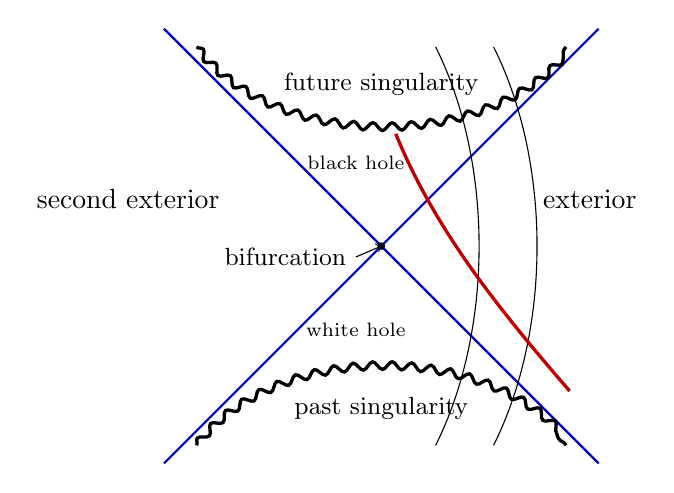
\begin{tikzpicture}[scale=0.92]
\draw[blue!75!black,thick] (-3,-3) -- (3,3);
\draw[blue!75!black,thick] (-3,3) -- (3,-3);
\draw[very thick,decorate,decoration={snake,amplitude=1.4pt,segment length=7pt}]
  (-2.55,2.75) .. controls (-1.45,1.35) and (1.45,1.35) .. (2.55,2.75);
\draw[very thick,decorate,decoration={snake,amplitude=1.4pt,segment length=7pt}]
  (-2.55,-2.75) .. controls (-1.45,-1.35) and (1.45,-1.35) .. (2.55,-2.75);
\draw (0.75,-2.75) .. controls (1.55,-1.15) and (1.55,1.15) .. (0.75,2.75);
\draw (1.55,-2.75) .. controls (2.35,-1.15) and (2.35,1.15) .. (1.55,2.75);
\draw[red!75!black,very thick] (2.6,-2.0) .. controls (1.65,-0.9) and (0.75,0.2) .. (0.2,1.55);
\fill (0,0) circle (1.5pt);
\node[above,font=\small] at (0,1.95) {future singularity};
\node[below,font=\small] at (0,-1.95) {past singularity};
\node[right] at (2.10,0.65) {exterior};
\node[left] at (-2.10,0.65) {second exterior};
\node[font=\scriptsize] at (-0.35,1.15) {black hole};
\node[font=\scriptsize] at (-0.35,-1.15) {white hole};
\node[font=\small,anchor=east] (bifurcation-label) at (-0.35,-0.15) {bifurcation};
\draw[->,thin] (bifurcation-label.east) -- (0,0);
\end{tikzpicture}
\caption{整理後的未緊緻化因果圖。零測地線視界在分叉面交會；類空奇點則位於未來與過去的楔形區域。}
\end{figure}

\subsection{可能，不代表典型}

微觀力學在極佳近似下具有時間反演不變性，但宏觀歷史卻有偏好的方向。炸彈很容易爆炸，散落的碎片卻幾乎不會重新聚攏，把炸彈重建起來。球很容易從不穩定的頂點滾落，隨手拋出的球卻幾乎不會恰好停在那裡。排列成三角形的撞球很容易散開，散開的球卻不會自發排回原來的形狀。冰塊會在熱水中融化，水卻幾乎不會自行排出一塊重新形成的冰。

差別在於熵。低熵宏觀態只占據相空間中的極小區域；高熵宏觀態則包含極大量的微觀排列。方程容許反向軌跡，但要製備相應的初始微觀態，需要極其精確的關聯。

\begin{classroomqa}
\audiencequestion{每一種精確的散射構型，難道不都和其精確的時間反演構型一樣不可能嗎？\lecturetimestamp{00:56:55}}
\lecturerresponse{若逐一指定微觀態，確實如此。比較宏觀態時才會出現不對稱。一種散開的排列所包含的微觀態，遠多於一個精確排列好的三角形；因此，幾乎所有符合前一種描述的微觀態，在宏觀上仍是無序的。}
\end{classroomqa}

白洞若要放出一個組織完整的愛麗絲，就是這類熵降低歷史的引力版本。可逆方程容許這種歷史，但它需要極其特殊的過去。視界本身具有熵，並隱含微觀資訊，因此並非邏輯上不可能出現一個愛麗絲大小的漲落；只是這種情況受到極強的抑制。

\begin{classroomqa}
\audiencequestion{這種漲落會是量子漲落還是熱漲落？\lecturetimestamp{00:59:48}}
\lecturerresponse{兩者都可能有所貢獻。在一般的熱系統中，主要以熱漲落來描述；對黑洞而言，量子效應與熱效應彼此交織。無論是哪一種，核心的抑制因素都是熵。}
\end{classroomqa}

\section{固有距離與彭羅斯緊緻化}

繪製整體時空之前，先把徑向相關術語說清楚。固有時是時鐘沿類時世界線所量得的時間。固有距離則是一串局部米尺沿選定類空曲線所量得的距離。對於史瓦西時空的固定\(t\)切片，
\begin{equation}
d\rho=\frac{dr}{\sqrt{1-2GM/r}}.
\label{eq:l04-proper-distance}
\end{equation}
因此，\(r\)是面積座標，並非從視界量起的直接尺量距離。

現在從徑向平直時空開始，只保留\(t\)與\(\rho\ge0\)。直線\(\rho=0\)是空間原點。徑向光線若朝原點傳播，便會從原點另一側繼續向外；在約化的半平面圖中，這看起來像是反射。

彭羅斯圖將\(t\)與\(\rho\)的所有有限和無限取值映射至有限區域，同時保留零方向。作圖有兩項規則：
\begin{enumerate}
\item 將整個時空緊緻化為有限區域；
\item 使徑向光線維持在\(45^\circ\)。
\end{enumerate}
長度和一般角度會改變；因果關係則保持不變。

\begin{figure}[htbp]
\centering
\includegraphics[width=0.70\textwidth]{lecture_04_figure_06.png}
\caption{徑向 Minkowski 時空的完整緊緻化網格。無限時間位於左上與左下端點，無限半徑則被壓縮至右側尖端。}
\lectureframe{01:14:44.040}
\end{figure}

\begin{figure}[htbp]
\centering
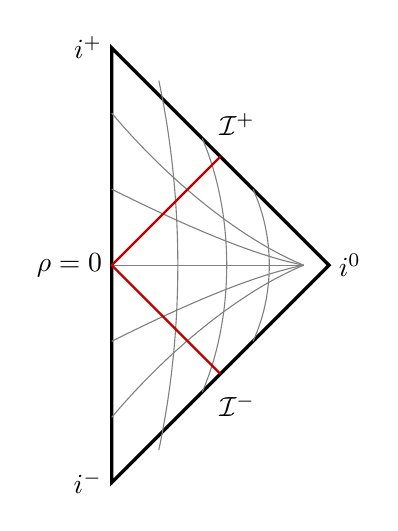
\begin{tikzpicture}[scale=0.92]
\coordinate (im) at (0,-3);
\coordinate (ip) at (0,3);
\coordinate (iz) at (3,0);
\draw[very thick] (im) -- (ip) -- (iz) -- cycle;
\draw[gray] (0,-2.1) .. controls (0.8,-1.15) and (1.8,-0.35) .. (2.65,0);
\draw[gray] (0,-1.05) .. controls (0.9,-0.6) and (1.9,-0.15) .. (2.65,0);
\draw[gray] (0,0) -- (2.65,0);
\draw[gray] (0,1.05) .. controls (0.9,0.6) and (1.9,0.15) .. (2.65,0);
\draw[gray] (0,2.1) .. controls (0.8,1.15) and (1.8,0.35) .. (2.65,0);
\draw[gray] (0.65,-2.55) .. controls (1.0,-0.9) and (1.0,0.9) .. (0.65,2.55);
\draw[gray] (1.25,-1.75) .. controls (1.7,-0.7) and (1.7,0.7) .. (1.25,1.75);
\draw[gray] (1.95,-1.05) .. controls (2.25,-0.4) and (2.25,0.4) .. (1.95,1.05);
\draw[red!75!black,thick] (1.5,-1.5) -- (0,0) -- (1.5,1.5);
\node[left] at (ip) {\(i^+\)};
\node[left] at (im) {\(i^-\)};
\node[right] at (iz) {\(i^0\)};
\node[above right] at (1.35,1.65) {\(\mathcal{I}^+\)};
\node[below right] at (1.35,-1.65) {\(\mathcal{I}^-\)};
\node[left] at (0,0) {\(\rho=0\)};
\end{tikzpicture}
\caption{有限三角形中的徑向 Minkowski 時空。紅色零線從\(\mathcal{I}^-\)進入，抵達原點後，再由\(\mathcal{I}^+\)離開。}
\label{fig:l04-flat-penrose}
\end{figure}

這些端點各有不同的因果意義：
\begin{equation}
\begin{aligned}
i^-&:\ \text{past timelike infinity},\\
i^+&:\ \text{future timelike infinity},\\
i^0&:\ \text{spatial infinity},\\
\mathcal{I}^-&:\ \text{past null infinity},\\
\mathcal{I}^+&:\ \text{future null infinity}.
\end{aligned}
\end{equation}
符號\(\mathcal{I}^{-}\)和\(\mathcal{I}^{+}\)分別讀作 scri minus 和 scri plus。

\begin{classroomqa}
\audiencequestion{零線是否應穿過每個變形網格單元的角點，因而略微彎曲？\lecturetimestamp{01:11:08}}
\lecturerresponse{若精確畫出完整的座標網格，其交點會與零曲線相符。關鍵在於這是共形構造：徑向零方向仍保持在\(45^\circ\)，即使固定\(t\)與固定\(\rho\)的網格線會彎曲、變得密集。}
\end{classroomqa}

\begin{classroomqa}
\audiencequestion{若光線沒有經過原點，該如何畫出它？\lecturetimestamp{01:11:45}}
\lecturerresponse{它會到達一個非零的最近距離，接著再向外傳播。保留角向運動後，它投影出的徑向路徑不一定是單一的直\(45^\circ\)線。}
\end{classroomqa}

\begin{classroomqa}
\audiencequestion{那麼，為什麼那條光線不沿\(45^\circ\)方向？\lecturetimestamp{01:12:49}}
\lecturerresponse{\(45^\circ\)這項規則說的是徑向光線。帶有角動量的零測地線，其部分運動分配在角方向上，因此它在\(t\)-\(\rho\)平面上的投影並非徑向。}
\end{classroomqa}

\section{永恆史瓦西因果圖}

緊緻化後的圖中有四個區域。兩側的菱形是漸近平坦的外部區域。上方三角形是黑洞內部，終止於未來類空奇點。下方三角形是白洞區域，起始於過去類空奇點。這些區域合在一起，構成最大延拓的史瓦西幾何。

\begin{figure}[htbp]
\centering
\includegraphics[width=0.74\textwidth]{lecture_04_figure_07.png}
\caption{黑板上繪出的完整永恆史瓦西彭羅斯圖，標示了奇點、視界、零軌跡，以及一個漸近邊界。}
\lectureframe{01:21:30.000}
\end{figure}

\begin{figure}[htbp]
\centering
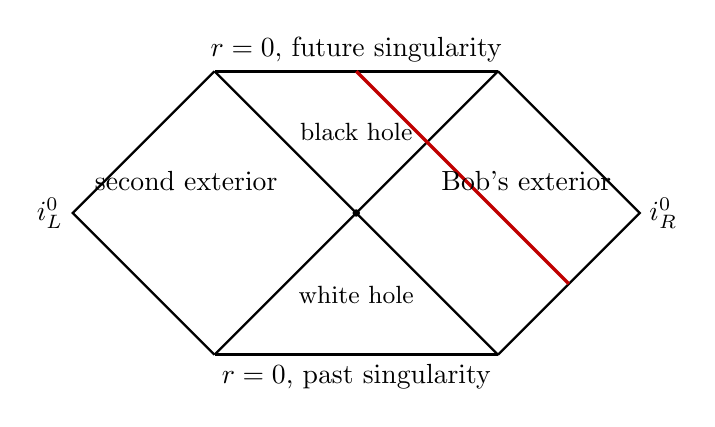
\begin{tikzpicture}[scale=0.90]
\coordinate (C) at (0,0);
\coordinate (TL) at (-2,2);
\coordinate (TR) at (2,2);
\coordinate (BL) at (-2,-2);
\coordinate (BR) at (2,-2);
\coordinate (L) at (-4.0,0);
\coordinate (R) at (4.0,0);
\draw[very thick] (TL) -- (TR);
\draw[very thick] (BL) -- (BR);
\draw[thick] (C) -- (TL) (C) -- (TR) (C) -- (BL) (C) -- (BR);
\draw[thick] (TL) -- (L) -- (BL);
\draw[thick] (TR) -- (R) -- (BR);
\draw[red!75!black,very thick] (3,-1) -- (1,1) -- (0,2);
\node[above] at (0,2) {\(r=0\), future singularity};
\node[below] at (0,-2) {\(r=0\), past singularity};
\node[font=\small] at (0,1.15) {black hole};
\node[font=\small] at (0,-1.15) {white hole};
\node at (2.4,0.45) {Bob's exterior};
\node at (-2.4,0.45) {second exterior};
\node[right] at (R) {\(i^0_R\)};
\node[left] at (L) {\(i^0_L\)};
\fill (C) circle (1.5pt);
\end{tikzpicture}
\caption{永恆史瓦西時空的四個區域。一條入射徑向光線穿過未來視界，終止於\(r=0\)。}
\label{fig:l04-eternal}
\end{figure}

一條從\(\mathcal{I}^-\)入射的徑向光線穿過未來視界，最後終止於奇點。上方三角形中的每條因果曲線都會有相同的結局。第二個外部區域常被描述為愛因斯坦--羅森橋的另一端，但這座橋無法穿越：任何試圖從一個外部區域因果地前往另一個外部區域的旅程，都會進入黑洞區域並抵達奇點。

\begin{classroomqa}
\audiencequestion{兩個外部世界是否由蟲洞連接？訊號能穿過去嗎？\lecturetimestamp{01:22:21}}
\lecturerresponse{在適當的空間切片上，永恆幾何包含一座愛因斯坦--羅森橋，但沒有因果訊號能從一個外部區域穿越到另一個。橋收縮得太快；即使是進入視界的光，也會終止於未來奇點。}
\end{classroomqa}

這張圖描述的是一個自始至終存在的黑洞。真實的天體物理黑洞由物質坍縮形成，其因果圖沒有過去白洞奇點，也沒有第二個漸近外部區域。要構造這種幾何，我們需要了解球殼。

\section{透過坍縮形成黑洞}

設想一個由入射粒子構成的稀疏球殼。這些粒子可以是光子：能量會產生引力，因此足夠集中的輻射脈衝能形成黑洞。坍縮前，中心區域近似於空的平直時空；足夠多的能量受到壓縮後，外部則近似於史瓦西時空。接下來要做的是沿著移動中的球殼，把這兩個區域接合起來。

\subsection{牛頓球殼定理}

對於總質量為\(M\)的球對稱牛頓球殼，引力的高斯定律為
\begin{equation}
\oint \mathbf{g}\cdot d\mathbf{A}=-4\pi G M_{\mathrm{enc}}.
\label{eq:l04-gauss-gravity}
\end{equation}
球對稱性使得\(\mathbf{g}=g(r)\hat{\mathbf r}\)，因此
\begin{equation}
g(r)=
\begin{cases}
0, & r<R_{\mathrm{shell}},\\[4pt]
-\dfrac{GM}{r^2}, & r>R_{\mathrm{shell}}.
\end{cases}
\label{eq:l04-shell-field}
\end{equation}
殼內沒有包圍的質量，引力場為零。殼外的引力作用則完全等同於中心有一個點質量\(M\)。殼內的位勢是常數，不是零，但局部的牛頓力為零。\editorialnote{課堂上以場線說明的論證，可由高斯定律精確表述。比較相對論中的時鐘歸一化時，零場與常數位勢之間的差別很重要。}

只要總質量守恆，完美球對稱的球殼即使在收縮，這項結論依然成立。改變的只有內部解與外部解之間的邊界位置。

\subsection{伯克霍夫定理}

相對論中的對應定理是伯克霍夫定理：任何球對稱的真空區域，在局部上都是史瓦西解族的一部分。對於中心沒有質量的球殼，
\begin{align}
ds^2_{\mathrm{inside}}&=-dT^2+dR^2+R^2d\Omega_2^2,\\
ds^2_{\mathrm{outside}}&=
-\left(1-\frac{2GM}{r}\right)dt^2
\nonumber\\
&\quad+\frac{dr^2}{1-2GM/r}
+r^2d\Omega_2^2.
\label{eq:l04-birkhoff-pieces}
\end{align}

\begin{figure}[htbp]
\centering
\includegraphics[width=0.74\textwidth]{lecture_04_figure_08.png}
\caption{球殼接合示意圖：圓內是平直時空，圓外是史瓦西解。}
\lectureframe{01:34:15.000}
\end{figure}

\begin{classroomqa}
\audiencequestion{在廣義相對論中，球殼外部的度規是什麼？\lecturetimestamp{01:33:17}}
\lecturerresponse{是史瓦西度規，其質量參數等於球殼的總守恆質量。空無一物的中心區域，在局部上是閔可夫斯基時空。}
\end{classroomqa}

\begin{classroomqa}
\audiencequestion{球殼收縮時，為什麼質量參數不會改變？\lecturetimestamp{01:34:33}}
\lecturerresponse{因為總能量守恆。球殼半徑以及動能或束縛能的貢獻可以改變，但孤立球對稱系統的守恆外部質量固定不變。移動中的球殼改變的是平直區域與史瓦西區域的接合位置。}
\end{classroomqa}

內部平坦，並不表示內部時鐘必然與無窮遠處的時鐘採用相同的歸一化。跨越殼層進行匹配時，內部時間座標可能會乘上一個常數；若殼層正在運動，則還須滿足相應的接合條件。\editorialnote{伯克霍夫定理分別確定各真空區域的局部時空幾何。兩區域座標之間的整體關係，則由跨越殼層匹配誘導度規與外曲率來決定。這些細節暫且略過，正如殼層坍縮的構造也留待下一講再談。}

現在，我們已具備描述黑洞形成所需的兩個部分：收縮殼層內部的閔可夫斯基時空，以及殼層外部的施瓦西時空。殼層向內移動時，兩者的交界面描繪出一條世界管。追蹤這條世界管穿越原本的施瓦西半徑，就能以規則的坍縮前區域取代圖~\ref{fig:l04-eternal}中不合物理的過去半部，並揭示真實黑洞的事件視界從何處開始形成。
